\appendix
\renewcommand\thefigure{\thesection.\arabic{figure}}
\setcounter{figure}{0}
\begin{center}
\textsc{\huge Appendix}\vspace*{.5cm} \\
\textbf{\Large Firm and Worker Dynamics in a Frictional Labor Market}\vspace*{.5cm} \\
\emph{\Large Adrien Bilal, Niklas Engbom, Simon Mongey, Gianluca Violante}\vspace*{.5cm} \\
\end{center}

\noindent This Appendix is organized as follows.
Section \ref{appx:staticexample} provides intuition for how our assumptions \textbf{(A)} yield a tractable Bellman equation for joint value.
Section \ref{appx:S_characterization} provides a characterization of the surplus function.
Section \ref{appx:CRS_limit} derives an alternative limit of the Bellman equation for the joint value as decreasing returns vanish.
Section \ref{appx:limiting_economies} derives the limiting behavior of our economy when frictions vanish.
Section \ref{appx:identification} illustrates identification of the model.

\section{Static Example}
\label{appx:staticexample}

\paragraph{Set up.}
Consider a firm with decreasing returns to scale technology $y(z,n)$ such that $y(z,0) = 0$. Suppose the firm starts with productivity $z$ and $n=1$ worker. The current contract between the firm and the incumbent specifies a wage $w_{1}\in (b,y(z,1))$, where $b=U$ is the value of unemployment.
At this point, the incumbent worker does not have a credible threat to quit into unemployment nor the firm has a credible threat to fire the worker. Then, the labor market opens. For now we also assume that the firm has sunk the cost of a vacancy $c$. Later we explicitly consider the decision to post a vacancy.

\subsection{$UE$ hire}
\label{appx:UE_hire}
We describe how to obtain the `UE hire' term  in \eqref{eq:JointValue}.
Assume the firm's vacancy meets an unemployed worker.
Four different cases can arise from the combination of hiring/not hiring and renegotiating/not renegotiating the wage with the incumbent.
Our assumption on external negotiation \textbf{(A-EN)} requires that in all cases the take-leave wage offer of the firm to the outside worker is $w_{2}=b$. Our internal negotiation assumption \textbf{(A-IN)} requires that the joint value with and without renegotiation is the same and simply equals output $y(z,n)$. Let $w_{1}^{\ast }$ be the incumbent wage after the internal negotiation.

If the firm hires the new worker, its profits are as follows:
\vspace{-.3cm}\begin{equation*}
\underbrace{\Big.
y(z,2)-w_{1}-b\Big.}_{\text{Without renegotiation}}\quad,\quad
\underbrace{\Big.
y(z,2)-w_{1}^{\ast }-b\Big.}_{\text{With renegotiation}}\:,
\vspace{-.3cm}\end{equation*}%
If the firm does not hire the new worker, its profits are
\vspace{-.3cm}\begin{equation*}
\underbrace{\Big.
y(z,1)-w_{1}\Big.}_{\text{Without renegotiation}}\quad,\quad
\underbrace{\Big.
y(z,1)-w_1^\ast\Big.}_{\text{With renegotiation}}
\vspace{-.3cm}\end{equation*}%
We now describe which case occurs.
This requires understanding when our mutual consent assumption \textbf{(A-MC)} coupled with limited commitment on layoffs \textbf{(A-LC)} bind. In particular, the firm may obtain a credible threat to trigger renegotiation of $w_1$. We focus first on when a hire occurs.

\vspace*{-.3cm}
\paragraph{Hire.}
A hire \emph{without} renegotiation occurs when the following two conditions hold:
\vspace*{-.3cm}\begin{equation}
\underbrace{\Big.
y(z,2) - w_1 - b \geq y(z,1) - b
\Big.}_{\text{No credible threat}}  \quad,\quad
\underbrace{\Big.
y(z,2) - w_1 - b \geq y(z,1) - w_1
\Big.}_{\text{Optimal to hire w/o renegotiation}}  \label{eq:S_hu_1}
\vspace*{-.3cm}\end{equation}
The first condition illustrates that the threat to fire the incumbent worker is not credible, which under \textbf{(A-MC)} implies no renegotiation. Keeping the incumbent worker at $w_{1}$ and employing the outside worker at $b$ delivers a higher value to the firm than the threat of ``swapping'':
firing worker one and hiring the unemployed worker in his place.
Given no renegotiation, the second condition ensures hiring is privately optimal for the firm.

A hire \emph{with} renegotiation occurs when the following two conditions hold:
\vspace*{-.3cm}\begin{equation}
\underbrace{\Big.
y(z,2) - w_1 - b < y(z,1) - b
\Big.}_{\text{Credible threat}}  \quad,\quad
\underbrace{\Big.
y(z,2) - w_1^* - b > y(z,1) - w_1^*
\Big.}_{\text{Optimal to hire w/ renegotiation}} .  \label{eq:S_hu_2}
\vspace*{-.3cm}\end{equation}
The firm has now a credible threat to fire the incumbent worker according to \textbf{(A-LC)}. This is possible only under decreasing returns to scale: even though $w_1<y(z,1)$, the first inequality in \eqref{eq:S_hu_2} implies $w_1>y(z,2)-y(z,1)$, i.e. the incumbent wage is above its own marginal product. Employing the outside worker at $b$ and keeping the incumbent worker at $w_{1}$ delivers a lower value than `firing and swapping'. The second condition is necessary for hiring to be optimal under the renegotiated wage $w_1^*$ to the incumbent worker.

Under the zero sum game assumption \textbf{(A-IN)}, the renegotiated wage $w_1^*$ only redistributes value between the incumbent worker and the firm, but does not affect total value.\footnote{Two relevant cases that would violate this condition are
    (i) if worker's effort depends on the wage and enters the production function, and
    (ii) concave utility.} In addition, it must be individually rational, and so $w_1^\ast\in[b,y(z,2)-y(z,1)]$. Without further assumptions we cannot say where exactly the new wage lies within this interval, but we can nonetheless pin down allocations.

Rearranging the optimal hiring conditions, we observe that both are satisfied as long as
\vspace*{-.3cm}\begin{equation}
y(z,2)-y(z,1)>b. \label{eq:S_hu_3}
\vspace*{-.3cm}\end{equation}
Note that without internal renegotiation {\bf(A-IN)}, the hiring condition would differ in the two cases. If wages could not be cut and the firm had a credible threat, the incumbent worker would be fired and the firm would always hire the unemployed worker ($y(z,1)>b$). As a result, to determine firm size next period, one would need to know the incumbent's wage to distinguish between the two cases (thus, in the general model with $n$ workers, the whole wage distribution). Similarly, if a fraction of output were to be lost because of the internal negotiation, a violation of {\bf(A-IN)}, the hiring conditions in \eqref{eq:S_hu_1} and \eqref{eq:S_hu_2} would differ and, again one would need to know wages to determine whether a hire occurs.

We can write inequality \eqref{eq:S_hu_3} in terms of joint value.
Workers' values are simply equal to their wage $w_i$ for $i\in\{1,2\}$. The firm's value is simply equal to its profits. The fact that wages are valued linearly by both worker and firm implies that the joint value $\Omega(z,n)$ is independent of wages:
\vspace*{-.3cm}\begin{equation*}
\Omega \left(z,n\right) = \underbrace{ y(z,n) - \sum_{i=1}^{n} w_i  }_\text{Firm value} \quad  + \underbrace{ \sum_{i=1}^{n} w_i }_\text{Sum of workers' values}
\quad,\quad\text{for any }\left(w_i\right)_{i=1}^n.
\vspace*{-.3cm}\end{equation*}
Using the definition of joint value, equation \eqref{eq:S_hu_3} characterizes when the UE hire occurs:
\vspace*{-.3cm}\begin{equation}\label{eq:S_hu_omega}
\Omega \left( z,2\right) -\Omega \left( z,1\right) > U.
\vspace*{-.3cm}\end{equation}%
Thus, the decision of hiring from unemployment does not depend on wages, but only on productivity, size, and the value of unemployment $U=b$.

\vspace*{-.3cm}
\paragraph{No hire.}
Consider now the cases where no hiring occurs. Recall that, once an unemployed worker is met, the firm has always a credible threat against the incumbent since $w_1>b$. No hire with renegotiation therefore occurs when the following two conditions hold:
\vspace*{-.3cm}\begin{equation}\label{eq:S_hu_nohire}
\underbrace{\Big.
y(z,1) - b > y(z,1) - w_1
\Big.}_{\text{Credible threat}} \quad,\quad
\underbrace{\Big.
y(z,1) - w_1^* \geq y(z,2) - w_1^* - b
\Big.}_{\text{Optimal to not hire}}
\vspace*{-.3cm}\end{equation}
After renegotiation the incumbent wage is driven down to $w_1^{\ast}$. Since this outcome represents a redistribution of value between firm and worker then, consistent with $\textbf{(A-IN)}$, the joint value remains $\Omega(z,1)$.\footnote{
    The value before renegotiation was $\Omega \left( z,1\right) =z-w_{1}+w_{1}=z$.
    The joint value after renegotiation is $\Omega \left( z,1\right) =z-w_1^*+w_1^*=z$.}
Finally, the no-hiring condition in \eqref{eq:S_hu_nohire} can be re-written as in \eqref{eq:S_hu_3} with the opposite inequality, $\Omega(z,2) - \Omega(z,1) \leq U$.

\vspace*{-.3cm}
\paragraph{Combined.}
The firm hires from unemployment when the \emph{marginal value} of the job seeker exceeds the value of unemployment:
\vspace*{-.3cm}\begin{equation}
\frac{\Omega \left( z,2\right) -\Omega \left( z,1\right)}{2-1} >U.
\vspace*{-.3cm}\end{equation}%
In addition, the joint value of the firm and its workers rises by $\frac{\Omega \left( z,2\right) -\Omega \left( z,1\right)}{2-1} - U$ when the hire occurs. This is exactly the \emph{$UE$ hire} term in the HJB equation \eqref{eq:JointValue}.
In the case of a hire, incumbent wages may or may not be renegotiated but this has no impact on whether hiring occurs, or how the joint value changes.
When this condition fails, the firm does not hire, wages are renegotiated, but the joint value remains constant.
All decisions require knowledge of $(z,n)$ only, but not of incumbents' wages.

We now generalize the $UE$ hire case analyzed in the main text to a firm with multiple incumbents.

\vspace*{-.2cm}\subsection{\emph{$UE$ hire} when the internal renegotiation involves multiple workers}
\label{appx:UE_hire_multiple}
It is sufficient to consider the case of two incumbent workers, $n=2$. Without loss of generality, assume that the second worker is paid more than the first, $w_{2}>w_{1}$. As in the approach taken earlier, suppose the firm has posted a vacancy that has met an unemployed worker.
We have three cases to consider which illustrate how the firm may use a worker outside the firm to sequentially renegotiate wages of workers inside the firm.

First, the firm hires \emph{without} renegotiation if:
\vspace*{-.3cm}\begin{equation*}
\underbrace{\Big.
y(z,3)-w_{1}-w_{2}-b > y(z,2)-w_{1}-b
\Big.}_{\text{No credible threat to $w_2$}}
\quad,\quad
\underbrace{\Big.
y(z,3)-w_{1}-w_{2}-b > y(z,2)-w_{1}-w_{2}
\Big.}_{\text{Optimal to hire under $(w_1,w_2)$}}.
\vspace*{-.3cm}\end{equation*}
Hiring with current wages is preferred to replacing the most expensive incumbent---there is no credible threat---, and given no renegotiation, hiring is optimal.
Since $w_2>w_1$, no credible threat to worker 2 implies no credible threat to worker 1.

\noindent Second, the firm hires \emph{with} renegotiation with worker 2 if:
\vspace*{-.3cm}\begin{equation*}
\underbrace{\Big.
y(z,2)-w_1-b>y(z,3)-w_{1}-w_{2}-b >y(z,2)-w_2-b
\Big.}_{\text{Credible threat for worker 2 only}}
\quad,\quad
\underbrace{\Big.
y(z,3)-w_{1}-w_{2}^{\ast}-b>y(z,2)-w_1-w_2^*
\Big.}_{\text{Optimal to hire under $(w_1,w_2^\ast)$}}.
\vspace*{-.3cm}\end{equation*}%
The threat is credible for worker 2, but is not for worker 1, and, conditional on renegotiating to $(w_1,w_2^\ast)$, hiring is optimal.

\noindent Third, the firm hires \emph{with} renegotiation with \emph{both} workers if:
\vspace*{-.3cm}\begin{equation*}
\underbrace{\Big.
y(z,2)-w_1-b>y(z,2)-w_2-b>y(z,3)-w_1-w_2-b
 \Big.}_{\text{Credible threat for both workers}}
\quad,\quad
\underbrace{\Big.
y(z,3)-w_{1}^{\ast}-w_{2}^{\ast}-b>y(z,2)-w_{1}^{\ast}-w_{2}^{\ast}
\Big.}_{\text{Optimal to hire under $(w_1^{\ast},w_2^{\ast})$}}.
\vspace*{-.3cm}\end{equation*}%
In all three cases, the optimal hiring condition can be written in terms of joint value as:
\vspace*{-.3cm}\begin{equation}
\frac{\Omega(z,3)-\Omega(z,2)}{3-2} > U.\label{UEhire_multiple}
\vspace*{-.3cm}\end{equation}
This last inequality does not depend on the order of the internal negotiation between firm and workers. In conclusion, the distribution of wages among incumbents again determines the patterns of wage renegotiation, but is immaterial for the sufficient condition for hiring. Hiring occurs whenever the marginal value of adding a worker to the coalition exceeds the value of unemployment.

Assumption \textbf{(A-LC-c)} that was not present in the one worker example plays a role here. Suppose that the renegotiated wage for worker 2 is pushed all the way down to $b$, making her indifferent between staying and quitting. Worker 1 could transfer a negligible amount to worker 2 in exchange of her quitting, which would raise the firm's marginal product and, possibly, remove its own threat. This is problematic for the representation because in this latter case the hiring condition becomes $y(z,2)-w_{1}-b>y(z,1)-w_{1}$, distinct from \eqref{UEhire_multiple}. Thus, to know whether a firm hires or not, one would need to know the wage distribution inside the firm.  \textbf{(A-LC-c)} is sufficient to rule out transfers among workers and to prevent this scenario from happening.

Note that this transfer scheme between workers occurring during the internal negotiation changes the joint value, and hence one can think of \textbf{(A-LC-c)} as being subsumed into  \textbf{(A-IN)} already.

In what follows we return to the case where the firm has only one worker.

\subsection{\emph{$EE$ hire}}
Now suppose that the worker matched with the firm's vacancy is currently employed at another firm with productivity $z^{\prime}$ and a single worker $n'=1$.
The situation is not that different from \emph{$UE$ hire}, except that the potential hire may have a better outside option in the form of the retention offer made to her by her current employer under \textbf{(A-EN)}.
To see the similarity for now we fix this wage offer at $\overline{w}$.
The same four cases described in section \ref{appx:UE_hire} can arise, except with $\overline{w}$ playing the role of $b$.\footnote{Renegotiation will happen for different values of $w_1$ in the no hire case. Indeed, to establish the presence of a credible threat $w_1$ must be compared to $\overline{w}$ instead of $b$, but this has no allocative implications for the hiring decisions.}
We can therefore reason as before and jump to the result that hiring will occur if and only if the following counterpart to \eqref{eq:S_hu_omega} holds:
\vspace*{-.3cm}\begin{equation*}
\Omega(z,2) - \Omega(z,1) > \overline{w}.
\vspace*{-.3cm}\end{equation*}

We now determine the poached worker's outside option $\overline{w}$.
The poached firm's willingness to pay is a wage $\widetilde{w}$ that makes it indifferent between retaining and releasing the worker: $y(z',1) - \widetilde{w} = 0$.
Hence, the contacted worker 
switches to the new employer as long as the poaching firm offers $\overline{w} \geq \widetilde{w} = y(z',1)$.
Bertrand competition between the two firms implies that the poaching firm offers $\overline{w}=y(z^\prime,1)$, which is exactly the marginal value of the worker at the poached firm. As in the case of \emph{$UE$ hire}, whether \emph{$EE$ hire} occurs can be summarized by joint values:
\vspace*{-.1cm}\begin{equation} \label{eq:S_he_omega}
\frac{\Omega \left( z,2\right) -\Omega \left( z,1\right)}{2-1} >
\frac{\Omega \left( z^{\prime},1\right) -\Omega \left( z^{\prime },0\right)}{1-0}.
\end{equation}
The \emph{$EE$ hire} decision is entirely characterized by knowledge of the pair $(z,n)$ for the two firms.\footnote{
    The case when the firm meets a worker at a firm with $(z^\prime,2,w_1,w_2)$ is similar.
    Suppose the firm meets worker 1.
    The poached firm has the additional option of cutting $w_2$, but this is inconsequential for the argument because it only redistributes value within the poached-from firm.
    }  The value gain to the firm and its workers is the difference between the left-hand side and right-hand side of equation \eqref{eq:S_he_omega}. This comparison of marginal values is precisely the \emph{$EE$ hire} term in the HJB equation (1).

Finally, this exercise explains the absence of a \emph{$EE$ quit} term in \eqref{eq:JointValue}.
The payment received by its poached worker is equal to the poached coalition's willingness to pay, which is in turn exactly equal to the worker's marginal value to the coalition.
The joint value of the poached coalition therefore does not change as it loses its worker.
\emph{$EE$ quit} events play an important role in the dynamics of employment at the firm, but no role in the dynamics of $\Omega(z,n)$.

\subsection{Vacancy posting \label{static:vacancies}}
Up to this point we assumed that a meeting between a hiring firm and a job seeker had already occurred. We now turn to the vacancy posting decision and explain why \textbf{(A-VP)} is crucial for tractability.

Recall that in the hiring scenarios just analyzed, two cases arise when the firm can credibly force a wage cut: (i) when it hires and the incumbent wage is above the post-hire new marginal product; (ii) when hiring is not profitable, but the firm can credibly `fire and swap', i.e. as long as the reservation wage of the external worker met through search is below the incumbent wage.
The firm has therefore incentives to spend resources on vacancy posting for the sole purpose of transfering value between agents, a privately inefficient outcome. The amount spent would depend on the incumbent's wage, breaking the tractability of our representation. Private efficiency reinstates tractability.

We start with the firm's preferred vacancy policy.
Without loss of generality, suppose firms only meet unemployed workers (hence, upon a meeting, the `fire and swap' threat is always credible). The generalization to the case where the worker contacted can be either unemployed or employed is straightforward.
Let $v$ be the number of vacancies posted, $c(v)$ the associated cost, and $q v$ the probability a single vacancy meets a single worker.
If no meeting occurs, then as per \textbf{(A-MC)}, $w_1$ does not change so the value of the firm 
does not change.
The firm maximizing the expected return from vacancy posting  net of costs is:
\vspace*{-.3cm}\begin{eqnarray*}
\max_v & & 
- c(v) + qv \Big[\max \Big\{\underbrace{\Big.
y(z,2) - w_1^{\prime} - b\Big.}_{\text{Hire (cases 1\&2)}}
\:,\:
\underbrace{\Big.
y(z,1) - b\Big.}_{\text{No hire (case 3)}}
\Big\} - 
\Big( y(z,1) - w_1 \Big) \Big] \quad, 
\vspace*{-.5cm}\end{eqnarray*}
Following a meeting, three cases may occur.
In \textbf{Case 1}, the firm hires and there is no renegotiation, $w_1^\prime =w_1$. This case arises when the wage of the incumbent worker is low enough. Then, adding a second worker does not reduce the marginal product of labor down to the point where the firm has a credible layoff threat. In \textbf{Case 2}, the firm hires but the wage of the incumbent is renegotiated down to $w_1^\prime =w_1^\ast$. In this case, diminishing marginal returns drive the marginal product of labor with two workers below the incumbent's initial wage. In \textbf{Case 3}, the firm is better off not hiring, but under the threat of swapping out the incumbent, renegotiates $w_1$ down to $b$.
The firm's preferred vacancy policy $v^f$ then equates marginal cost to marginal expected return:
\vspace*{-.3cm}\begin{equation}\label{eq:VacancyFOC}
c_v\left(v^f
\right) =q
\Big[\max \Big\{y(z,2) - w_1^{\prime} - b
\:,\:
y(z,1) - b
\Big\} - \Big( y(z,1) - w_1 \Big) \Big].
\vspace*{-.3cm}\end{equation}
The first-order condition \eqref{eq:VacancyFOC} highlights that the firm's preferred vacancy policy depends on the incumbent's wage $w_1$ because this wage determines the gains from forcing a renegotiation through vacancy posting. This dependence is a source of intractability because, in the general model with $n$ workers, \eqref{eq:VacancyFOC} would depend on the entire wage distribution inside the firm.

Our assumption \textbf{(A-VP)} ensures that firms do not post $v^f$, but instead post the privately efficient amount of vacancies which does not depend on worker wages. We now show how our micro-foundation \textbf{(A-VPI)} implements \textbf{(A-VP)}.

\vspace*{-.2cm}\paragraph{Case 1 -- Hire without renegotiation.}
In this case the outcome is already \emph{privately efficient}. The worker's value does not decrease ($w_1^{\prime}=w_1$), and by the fact that a hire occurs, the firm's value must increase. We can also write the expected return as $qv\left[\Omega(z,2)-\Omega(z,1) - U\right]$. Since the return is independent of $w_1$, then the efficient vacancy policy is independent of $w_1$. The firm is choosing vacancies as if it were maximizing the joint surplus without having to appeal to additional assumptions.

In cases 2 and 3, the outcome is \emph{privately inefficient} because the firm may profit from vacancies that, if met by a job seeker, deliver a credible threat to cut the incumbent's wage to $w_1^\prime <w_1$.

Our assumption \textbf{(A-VPI)} allows the worker to correct for this over-posting by conceding a single pay cut in exchange for an alternative level of vacancies.\footnote{
    A pay cut regardless of the outcome of the search for a new worker maps exactly into a transfer from worker to firm, which is how we approach the proof.
    Promising \emph{state-contingent} wage cuts that depend on who the firm meets or whether a meeting occurs is not possible given our assumption of what is verifiable and contractible.
    Even if these states were verifiable, the result would only be for the worker to offer a menu of wage-cuts across states.
    This would increase worker value but not change allocations, hence for consistency with the rest of our assumptions, we assume a single wage cut.
}
The firm will accept this wage cut and choose the worker's preferred vacancies if it delivers at least the value obtained under the firm's preferred vacancies $v^f$. We show that the worker's preferred package satisfying incentive compatibility restores efficiency in vacancy posting.

\vspace*{-.2cm}\paragraph{Case 2 -- Hire with renegotiation.}
In this case, the incumbent's wage $w_1$ is high enough that the firm finds it profitable to raise the contact probability with an unemployed worker beyond what would be efficient. Although the hiring outcome is efficient ex-post, too much resources are spent on vacancies ex-ante. Let $w_1^{\ast}$ be the renegotiated wage after a meeting.
The worker chooses a package of vacancies and a wage cut in all states $(v^w,x)$ that solves:
\vspace*{-.3cm}\begin{eqnarray}
&&\max_{v^w,\:x}\:\: qv^w\Big(w_1^\ast - w_1\Big) - x
\label{eq:S_vac_mechdes} \\
\text{subject to}&&  \notag \\
&& q v^w \Big[ \Big( y(z,2) - (w_1-x) - b \Big) - \Big( y(z,1) - w_1 \Big) \Big] - c(v^w) \notag \\
&\geq & q v^f \Big[ \Big( y(z,2) - w_1^* - b \Big) \hspace{1.1cm} - \Big( y(z,1) - w_1 \Big) \Big] - c(v^f) \hspace{2cm}(IC) \notag
\vspace*{-.3cm}\end{eqnarray}
The worker anticipates that after a meeting their wage will be renegotiated to $w_1^\ast<w_1$. Given this wage cut, the worker seeks to limit the probability of this event by cutting back on vacancies. Incentive compatibility $(IC)$ requires that as the worker cuts vacancies it also cuts its wage so that the firm accepts the proposed policy $v^w$ over $v^f$.

The Pareto problem \eqref{eq:S_vac_mechdes} yields the result that vacancy posting is independent of $w_1$. First, given the linear objective function, $(IC)$ holds with equality. Thus, we can substitute out $x$. Second, the zero-sum game assumption \textbf{(A-IN)} implies that $w_1^\ast$ is a renegotiated wage that only redistributes value and hence drops out. Third, all terms that do not depend on $(x,v^w)$ are irrelevant to the worker's decision. Adopting the value notation, this leaves the following objective function:
\vspace*{-.3cm}\begin{equation*}
\max_{v^w}\:qv^w\Big[
\Big( \Omega(z,2) - U\Big)
-
\Omega(z,1) \Big]
\:-\: c\left(v^w\right).
\vspace*{-.3cm}\end{equation*}
The decision can therefore be characterized by the \emph{privately efficient return}, which is the change in joint value net of the cost of the new hire, $\Omega(z,2)-\Omega(z,1) - U$.

\vspace*{-.2cm}\paragraph{Case 3 -- No hire with renegotiation.}

In this case the `fire and swap' threat is credible. The incumbent's wage $w_1$ is high enough and the marginal product of an additional worker is below $b$. Replacing the return to hiring by the wage cut for the incumbent worker, the previous logic delivers 
\vspace*{-.3cm}\begin{equation*}
\max_{v^{w}}\:\:qv^{w}\:\Big[\Omega(z,1)-\Omega(z,1) \Big]\:-\: c\left(v^{w}\right)\quad\implies\quad v^w = 0
\vspace*{-.3cm}\end{equation*}
Absent the transfer from worker to firm, the firm would post positive vacancies $v^f$ even if the return from hiring is negative, i.e. $\Omega(z,2)-\Omega(z,1)<U$ to induce a wage cut, and $v^f$ would depend on $w_1$.
Under \textbf{(A-VPI)}, the worker takes a preemptive wage cut, and vacancies are zero, the efficient amount in this case.

\vspace*{-.2cm}\paragraph{Combined.}
Combining all three cases, 
privately efficient vacancies solve
\vspace*{-.3cm}\begin{equation*}
\max_{v}\: qv\:\left[\:\max\left\{ \frac{\Omega(z,2)-\Omega(z,1)}{2-1}-U,0\right\}\right] - c(v).
\vspace*{-.3cm}\end{equation*}

Note three properties of this solution.
First, the firm always hires when it meets an unemployed worker. Second, optimal vacancy posting equates the marginal gain in joint value to the marginal cost of a vacancy, and it only depends on $(z,n)$. Third, this condition is the flip-side of the separation frontier.
Expression \eqref{eq:JointValue} states that if $\Omega_n(z,n)> U$, then the firm will not separate with workers.
The terms inside the max expression say that if this is true, then the firm will post vacancies.\footnote{
    It is possible to determine the optimal wage cut $x$ that delivers the efficient policy, but throughout the paper we focus on allocations only.
    }

We conclude that under \textbf{(A-VPI)}, the joint value is sufficient to characterize the vacancy decision. The distribution of wages in the firm is immaterial.

\vspace*{-.2cm}\paragraph{Multiple incumbents.}
When the firm employs more than one worker, the efficient transfer scheme can be implemented by randomly selecting a worker under threat to offer a package  of wage-cuts and vacancies.
In exchange, the firm posts the efficient number of vacancies.
Under such a scheme, the initiating worker is strictly better off while the firm and the other workers are indifferent.
We establish this case in detail in Appendix II.

\subsection{Layoffs, quits, exit, entry}
Having described most of the terms in the HJB \eqref{eq:JointValue}, we conclude with the boundary conditions for exit, layoffs and  the free entry condition.

\vspace*{-.2cm}\paragraph{Layoffs.}
Consider now a firm with $n=2$ workers paid $(w_1,w_2)$, and assume that $w_{1}<y(z,1)$ such that worker 1 is never under threat of layoff.
The firm has a credible threat to fire worker $2$ if
\vspace*{-.3cm}\begin{equation*}
y(z,1) - w_1 > y(z,2)-w_1-w_2.
\vspace*{-.3cm}\end{equation*}
Such a situation may occur if, for example, productivity has just declined. The firm has a credible threat to negotiate down to a wage level $w_2^\ast$ such that 
$y(z,1) - w_1 = y(z,2) - w_1 - w_2^\ast$ and keep worker 2 employed.
From the worker's perspective, it is individually rational to accept any wage $w_2^\ast$ above $b$. Worker 2 is laid off if $y(z,1) - w_1>y(z,2) - w_1 -b$. In terms of joint value, this can be written in exactly the form of the layoff frontier \eqref{eq:Boundaries}:
\vspace*{-.2cm}\begin{equation*}
\frac{\Omega \left( z,2\right) -\Omega \left( z,1\right)}{2-1} < U.
\end{equation*}
The firm lays off workers until the marginal joint value of the worker is equal to the value of unemployment.\footnote{
    Note that, when both workers are under threat, the particular order in which values of workers are reduced is immaterial to the condition $\Omega \left( z,2\right) -\Omega \left(z,1\right) < U$.
    One could for example lower the wages of both workers proportionally, increasing the value of the firm, but a worker \emph{must} be fired if $y(z,2)-w_1^{\ast}-b < y(z,1)-w_1^{\ast}$ for any $w_1^{\ast}\geq b$.}
As noted earlier, this is the complement to the condition for posting vacancies. The special case with $n=1$ of this scenario also arises in the one worker-one firm model with productivity shocks of \citet{pvtearnings2010}.

\vspace*{-.2cm}\paragraph{Quits to unemployment.}
Since in this static model workers will accept a renegotiated wage down to $w_i^\ast=b$, they will only quit at the point where the firm has a credible threat to lower wages below $b$. This is exactly the point at which the marginal value is equal to the value of unemployment. In this sense \emph{layoffs} as described above are indistinguishable from quits to unemployment, as in any model with privately efficient separations. For ease of language all \emph{endogenous} $UE$ transitions are referred to as \emph{layoffs}, and we use \emph{quits} to refer only to $\emph{EE}$ transitions.

Finally, recall that in the dynamic model unemployed job seekers are promised a wage that implements a value $U$ to them. If events occur in the firm that reduce the continuation value to that worker below $U$ (e.g., a negative productivity shock), the incumbent may have a credible threat to quit and renegotiate her wage to restore its value at $U$, or above it, depending on the details of the internal negotiation. However, such renegotiation is, again, only a transfer of value within the firm. Separations remain privately efficient even in the dynamic model.

\vspace*{-.2cm}\paragraph{Exit.}
Now consider the exit decision of a firm with one worker. The private value of exit to the firm is the scrap value $\vartheta>0$. The firm therefore exits if and only if 
$y(z,1) - w_1^* <\vartheta$, where $w_1^\ast$ is a possibly renegotiated wage contingent on the firm remaining in operation.
If the profit from operating at the lowest possible renegotiated wage $w_1^\ast=b$ is greater than $\vartheta$, then the firm will continue to operate.
Hence, the firm exits if 
$y(z,1) - b <\vartheta$, and the renegotiated wage only affects the distribution of value.\footnote{
    The firm has no credible threat to reduce $w_1$ if $y(z,1)-w_1>\vartheta$.
    The firm can credibly threaten exit if $\vartheta\in\left(y(z,1)-w_1) ,y(z,1)-b\right)$, but in this case $w_1$ can be reduced to a point where this threat is no longer credible.
}
The exit condition can be written as $\Omega(z,1) - U < \vartheta$, and in the general case of $n$ workers is exactly the boundary condition in \eqref{eq:JointValue}: $\Omega \left( z,n\right) - nU < \vartheta.$

\vspace*{-.3cm}
\paragraph{Entry.}
Upon entry the firm has $n_0$ workers hired from unemployment. The private entry cost of the firm is $c_0$, so entry requires $\int y(z,n_0)d\Pi_{0}(z) - n_0 b > c_0$.
Using $\Omega(n,z) = y(z,n)$ and $U=b$, this requires $\int\Omega\left( z,n_0\right)d\Pi_{0}(z) > c_0 + n_0U$.

\subsection{From static to dynamic}
This static example showcases how to obtain every component of \eqref{eq:JointValue} from our set of assumptions.
Appendix II generalizes this proof to the dynamic case.
Two insights assist us.
First, the proof begins with a discrete workforce.
Here we are helped by continuous time, which removes complicated binomial probabilities of one, two, three, etc. incumbent workers meeting a competitor's vacancy.
Second, we take the continuous workforce limit of the discrete workforce HJB equation.
This limit delivers the joint value representation \eqref{eq:JointValue} in terms of the derivative of the joint value function rather than differences of values which, when moving up or down by one worker, are symmetric due to continuous differentiability.

\section{Characterization of surplus function}
\label{appx:S_characterization}

Here we prove the comparative statics on the surplus function $S(n,z)$ discussed in the main text.

\subsection{Hamilton Jacobi Bellman Variational Inequality for Total Value \label{appx:HJBVI}}
Before characterizing these conditions, we note that the joint value representation (1) and smooth-pasting boundary conditions that define the exit and layoff boundaries (2) are derived from solving the following Hamilton-Jacobi-Bellman-Variational-Inequality \citep[see][]{pham2009}, which we present here for completeness.
Its general formulation in terms of optimal switching between three regimes (operation, layoffs, exit)
on the entire positive quadrant, can be written as the following system:
\begin{eqnarray}\label{eq:AppHJBVI}
&& \max \Bigg\{ - \rho \Omega \left(z,n\right) + \max_{v \geq 0} -\delta n
[\Omega_n(z,n) - U] +q v \phi \left[ \Omega_n(z,n) -U \right] \\
&& \hskip1.2cm +q v \left( 1-\phi \right) \int \max\Bigg[\Omega_n(z,n) -
\Omega_n(z^{\prime},n^{\prime}) \ , \ 0 \Bigg]d\widetilde{H_n}\left(
z^{\prime},n^{\prime}\right) +\mu(z) \Omega_z(z,n) + \frac{\sigma(z)^2}{2}
\Omega_{zz}(z,n) \ ; \notag\\
&& \hskip1.3cm \underbrace{\vartheta + n U - \Omega(z,n)}_{\text{Exit}} \ ; \
\underbrace{\max_{k \in [0,n]}
\Omega(z,k) + (n-k) U - \Omega(z,n)}_{\text{Layoff}} \Bigg\} = 0 \hskip5mm , \hskip5mm
\forall (z,n) \in \mathbb{R}_+^2\notag
\end{eqnarray}
The HJBVI implies necessary ``value-matching'' and ``smooth-pasting'' boundary conditions: see \citet{brekkeoksendal1990}, \citet{peskirshiryaev2006} and \citet{stokey2009}.

Value matching conditions are standard, and simply state that the value function must be continuous at the exit and separation boundaries. Smooth pasting conditions obtain only when coalitions are actually crossing the exit or layoff boundaries. Intuitively, coalitions can then take an interior first-order optimality condition when they choose the stopping boundary. Thus, smooth pasting obtains either when there is volatility, or when the drift pushes coalitions outside of the continuation region.

Combining these observations, for exit, we have a value matching condition that holds for the entire boundary $n_E^*(z)$, and a smooth pasting condition in the $n$ direction that holds only where the drift is negative and firms actually exit.  We have a smooth pasting condition in the $z$ direction that holds for the entire boundary $n_E^*(z)$ because there is volatility in the $z$ direction. We collect these conditions in Conditions (iii) in Section 4.1.


\subsection{$S$ is increasing in $n$}

The no-endogenous-separations condition $S_n \geq 0$ implies
that the surplus is increasing in $n$.

\subsection{$S$ is increasing in $z$}

Re-write the problem in terms of $x = \log z$. Denote with a slight abuse of
notation $y(x,n) = y(e^x,n)$.
\begin{eqnarray*}
\rho S(x,n) &=& \max_{v \geq 0} y(x,n) - n b - c(v) \\
&+& [q \phi v - \delta n] S_n(x,n) + q (1-\phi) v \mathcal{H}(S_n(x,n)) \\
&+& \mu S_x(x,n) + \frac{\sigma^2}{2} S_{xx}(x,n)
\end{eqnarray*}
where we integrated by parts, and denoted $\mathcal{H}(s) = \int_0^s H_n(r)dr$%
. Denote $\zeta(x,n) = S_x(x,n)$. Differentiate the Bellman equation w.r.t. $%
x$ and use the envelope theorem to obtain
\begin{eqnarray*}
\rho \zeta(x,n) &=& y_x(x,n) \\
&+& \Big\{ \big[q \phi+q (1-\phi) H_n(S_n(x,n)) \big] v^*(x,n) - \delta n %
\Big\} \zeta_n(x,n) \\
&+& \mu \zeta_x(x,n) + \frac{\sigma^2}{2} \zeta_{xx}(x,n)
\end{eqnarray*}
Now consider the stochastic process defined by
\begin{eqnarray}  \label{stoc_proc_1}
dx_t &=& \mu dt + \sigma dW_t  \notag \\
dn_t &=& \Big\{ \big[q (1-\phi) H_n(S_n(x_t,n_t)) + q \phi \big] v^*(x_t,n_t)
- \delta n_t \Big\} dt
\end{eqnarray}
This correponds to the true stochastic process for productivity, but a
hypothetical process for employment, that in general differes from the
realized one. We can now use the Feynman-Kac formula (Pham 2009) to go back
to the sequential formulation:
\begin{eqnarray*}
\zeta(x,n) = \mathbb{E} \left[ \int_0^T e^{-\rho t} y_x(x_t,n_t) + e^{-\rho
T} \zeta(x_T,n_T) \ \Big| \ x_0 = x , n_0 = n , \{x_t,n_t\} \text{ follows (%
\ref{stoc_proc_1})} \right]
\end{eqnarray*}
and where $T$ is the hitting time of either the separation of exit region.
By assumption, $y_x > 0$, so the contribution of the first part is always
positive. On the exit region, smooth-pasting requires that $\zeta = 0$.
In the interior of the separation region, $\zeta = 0$. Under our regularity
assumption, we thus get $\zeta = 0$ on the layoff boundary. Thus,
\begin{eqnarray*}
\zeta(x,n) = \mathbb{E} \left[ \int_0^T e^{-\rho t} y_x(x_t,n_t)dt \ \Big| \
x_0 = x , n_0 = n , \{x_t,n_t\} \text{ follows (\ref{stoc_proc_1})} \right]
> 0
\end{eqnarray*}
which concludes the proof.

\subsection{$S$ is concave in $n$}

Denote $s(z,n) = S_n(z,n)$. Differentiate the Bellman equation w.r.t. $n$ on
the interior of the domain, use the envelope theorem and integrate by parts
to obtain:
\begin{eqnarray*}
(\rho+\delta) s(z,n) &=& y_n(z,n) - b \\
&+& \Big\{ \big[q \phi + q (1-\phi) H_n(s(z,n)) \big] v^*(z,n) - \delta n\Big\}
s_n(z,n) \\
&+& \mu(z) s_z(z,n) + \frac{\sigma^2(z)}{2} s_{zz}(z,n)
\end{eqnarray*}
Recall that
\begin{equation}
(1+\gamma) \bar{c} [ v^*(z,n) ]^\gamma = q \phi s(z,n) + q(1-\phi) \mathcal{H}%
(s(z,n))\label{appx_v*}
\end{equation}
In particular, differentiating w.r.t. $n$,
\begin{equation*}
\gamma (1+\gamma) \bar{c} [ v^*(z,n) ]^{\gamma-1} v^*_n(z,n) = \big[ q \phi +
q(1-\phi) H_n(s(z,n)) \big] s_n(z,n)
\end{equation*}
and so
\begin{equation*}
\gamma \frac{ v^*_n(z,n)}{v^*(z,n)} = \frac{\phi + (1-\phi) H_n(s(z,n))}{\phi
+ (1-\phi) \overline{H}(s(z,n))} \frac{s_n(z,n)}{s(z,n)}
\end{equation*}
where $\overline{H}(s) = \frac{\mathcal{H}(s)}{s} \leq 1$. Now denote $\zeta(z,n)
= s_n(z,n) = S_{nn}(z,n)$. Differentiate the recursion for $s$ w.r.t. $n$ to
obtain
\begin{eqnarray*}
&& \Bigg(\rho+ 2\delta - q (1-\phi) H_n^{\prime}(s(z,n) v^*(z,n)s_n(z,n) - q[
\phi + (1-\phi) H_n(s(z,n)) v_n^*(z,n) \Bigg) \zeta(z,n) \\
&=& y_{nn}(z,n) \\
&+& \Big\{ \big[\lambda \phi + \lambda (1-\phi) H_n(s(z,n) \big] v^*(z,n)-
\delta n\Big\}\zeta_n(z,n) \\
&+& \mu(z) \zeta_z(z,n) + \frac{\sigma^2(z)}{2} \zeta_{zz}(z,n)
\end{eqnarray*}
Now define the ``effective discount rate''
{\small
\begin{eqnarray*}
R(z,n, s_n(z,n)) &=& \rho+ 2\delta - q (1-\phi) H_n^{\prime}(s(z,n) v^*(z,n)
s_n(z,n) - q[ \phi + (1-\phi) H_n(s(z,n))] v_n^*(z,n) \\
&=& \rho+ 2\delta - q v^*(z,n) s_n(z,n) \underbrace{ \left\{ (1-\phi)
H_n^{\prime}(s(z,n)) + \frac{ \phi + (1-\phi) H_n(s(z,n))}{\gamma s(z,n)}\frac{%
\phi + (1-\phi) H_n(s(z,n))}{\phi + (1-\phi) \overline{H}(s(z,n))} \right\} }%
_{\equiv P(z,n) > 0}
\end{eqnarray*}}
where the second equality uses the expression for $v^*_n$ derived above.
Define the stochastic process
\begin{eqnarray}  \label{stoc_proc_2}
dz_t &=& \mu(z_t) dt + \sigma(z_t) dW_t  \notag \\
dn_t &=& \Big\{ \big[q (1-\phi) H_n(S_n(z_t,n_t)) + q \phi \big] v^*(z_t,n_t)
- \delta n_t \Big\} dt
\end{eqnarray}
As before, we can use the Feynman-Kac formula to obtain
\begin{eqnarray*}
\zeta(z,n) &=& \mathbb{E} \Bigg[ \int_0^T e^{- \int_0^t
R(z_\tau,n_\tau,\zeta(z_\tau,n_\tau)) d\tau} y_{nn}(z_t,n_t) dt +
e^{-\int_0^T R(z_\tau,n_\tau,\zeta(z_\tau,n_\tau)) d\tau T} \zeta(z_T,n_T) \\
&& \hskip6cm \Big| \ z_0 = z , n_0 = n , \{z_t,n_t\} \text{ follows (\ref%
{stoc_proc_2})} \Bigg]
\end{eqnarray*}
for $T$ the first hitting time of the exit/separation region. The
contribution of the first term is always negative. Note that $\zeta$ enters
in the effective discount rate. Inside the separation region and in the exit
regions, $\zeta = 0$. We restrict attention to twice continuously
differentiable functions, so $\zeta = 0$ on the exit and separation
frontiers. Then
\begin{eqnarray*}
\zeta(z,n) &=& \mathbb{E} \Bigg[ \int_0^T e^{- \int_0^t
R(z_\tau,n_\tau,\zeta(z_\tau,n_\tau)) d\tau} y_{nn}(z_t,n_t) dt \ \Big| \
z_0 = z , n_0 = n , \{z_t,n_t\} \text{ follows (\ref{stoc_proc_2})} \Bigg] <
0
\end{eqnarray*}
which concludes the proof.

\subsection{$S$ is supermodular in $(\log z, n)$}

Denote again $s(x,n) = S_n(x,n)$, where $x = \log z$. Recall that
\begin{eqnarray*}
(\rho+\delta) s(x,n) &=& y_n(x,n) - b \\
&+& \Big\{ \big[q \phi + q (1-\phi) H_n(s(x,n) \big] v^*(x,n) - \delta n\Big\}
s_n(x,n) \\
&+& \mu s_x(x,n) + \frac{\sigma^2}{2} s_{xx}(x,n)
\end{eqnarray*}
and that
\begin{equation*}
(1+\gamma) \bar{c} [ v^*(x,n) ]^\gamma = q \phi s(x,n) + q(1-\phi) \mathcal{H}%
(s(x,n))
\end{equation*}
In particular, differentiating w.r.t. $x$,
\begin{equation*}
\gamma \frac{ v^*_x(x,n)}{v^*(x,n)} = \frac{\phi + (1-\phi) H_n(s(x,n))}{\phi
+ (1-\phi) \overline{H}(s(x,n))} \frac{s_x(x,n)}{s(x,n)}
\end{equation*}
Now denote $\zeta(x,n) = s_x(x,n) = S_{xn}(x,n)$. Differentiate the
recursion for $s(x,n)$ w.r.t. $x$ to obtain
\begin{eqnarray*}
&& \Bigg(\rho+ \delta - q (1-\phi) H_n^{\prime}(s(x,n) v^*(x,n)s_x(x,n) - q[
\phi + (1-\phi) H_n(s(x,n)) v_x^*(x,n) \Bigg) \zeta(x,n) \\
&=& y_{nx}(x,n) \\
&+& \Big\{ \big[\lambda \phi + \lambda (1-\phi) H_n(s(x,n) \big] v^*(x,n)-
\delta n\Big\} \zeta_n(x,n) + \mu \zeta_x(x,n) + \frac{\sigma^2}{2} \zeta_{xx}(x,n)
\end{eqnarray*}
As before, define the ``effective discount rate''
{\small
\begin{eqnarray*}
R(x,n, s_x(x,n)) &=& \rho+ \delta - q (1-\phi) H_n^{\prime}(s(x,n) v^*(x,n)
s_x(x,n) - q[ \phi + (1-\phi) H_n(s(x,n))] v_x^*(x,n) \\
&=& \rho+ \delta - q v^*(x,n) s_x(x,n) \underbrace{ \left\{ (1-\phi)
H_n^{\prime}(s(x,n)) + \frac{ \phi + (1-\phi) H_n(s(x,n))}{\gamma s(x,n)}\frac{%
\phi + (1-\phi) H_n(s(x,n))}{\phi + (1-\phi) \overline{H}(s(x,n))} \right\} }%
_{\equiv P(x,n) > 0}
\end{eqnarray*}}
where the second equality uses the expression for $v^*_n$ derived above. As
before, define the stochastic process
\begin{eqnarray}  \label{stoc_proc_3}
dx_t &=& \mu dt + \sigma dW_t  \notag \\
dn_t &=& \Big\{ \big[q (1-\phi) H_n(S_n(e^{x_t},n_t)) + q \phi \big] %
v^*(x_t,n_t) - \delta n_t \Big\} dt
\end{eqnarray}
As before, we can use the Feynman-Kac formula to obtain
\begin{eqnarray*}
\zeta(x,n) &=& \mathbb{E} \Bigg[ \int_0^T e^{- \int_0^t
R(x_\tau,n_\tau,\zeta(x_\tau,n_\tau)) d\tau} y_{nx}(x_t,n_t) dt +
e^{-\int_0^T R(x_\tau,n_\tau,\zeta(x_\tau,n_\tau)) d\tau T} \zeta(x_T,n_T) \\
&& \hskip6cm \Big| \ x_0 = z , n_0 = n , \{x_t,n_t\} \text{ follows (\ref%
{stoc_proc_3})} \Bigg]
\end{eqnarray*}
for $T$ the first hitting time of the exit/separation region. The
contribution of the first term is always positive. Inside the separation
region and in the exit regions, $\zeta = 0$. We restrict attention to twice
continuously differentiable functions, so $\zeta = 0$ on the exit and
separation frontiers. Then
\begin{eqnarray*}
\zeta(x,n) &=& \mathbb{E} \Bigg[ \int_0^T e^{- \int_0^t
R(x_\tau,n_\tau,\zeta(x_\tau,n_\tau)) d\tau} y_{nx}(x_t,n_t) dt \ \Big| \
x_0 = z , n_0 = n , \{x_t,n_t\} \text{ follows (\ref{stoc_proc_3})} \Bigg]>0
\end{eqnarray*}
which concludes the proof.

\subsection{Net employment growth}
Denote again $s(z,n)=S_n(z,n)$. Net employment growth in the continuation region is
\begin{eqnarray*}
\frac{dn_t}{dt} &=& q \Big[ \phi + (1-\phi) H_n(s(z,n)) \Big] v^*(z,n) -
\lambda^E (1- H_v(s(z,n))) n - \delta n \equiv g(z,n)
\end{eqnarray*}
Using the expression the optimal vacancy condition $v^*(z,n)$ in \eqref{appx_v*}:
\begin{eqnarray*}
g(z,n) &=& \frac{q^{1+1/\gamma}}{[(1+\gamma) \bar{c}]^{1/\gamma}} \Big( \phi +
(1-\phi) H_n(s(z,n)) \Big) \Big( \phi s(z,n) + (1-\phi) \mathcal{H}%
(s(z,n)) \Big)^{1/\gamma} \\
&& - \lambda^E (1- H_v(s(z,n))) n - \delta n
\end{eqnarray*}
From the previous comparative statics on $S(z,n)$, it is straightforward
to see that $g(z,n)$ is increasing in $\log z$ and decreasing in $n$.

\section{Alternative CRS limit}
\label{appx:CRS_limit}
Consider the surplus equation \eqref{eq:finalBellmanS}. Assume $\alpha=1$, $\vartheta=0$ and vacancy costs homogeneous of degree one in $(v,n)$. Let $\nu=v/n$. In this case, the joint surplus is linear in $n$, $S(z,n) = \hat{S}(z)n$, where
\begin{eqnarray}
\label{eq:liserobin2}
(\rho+\delta) \hat{S}(z) &=& \max_{\nu\geq0}\:\: y(z) - b + q(\theta)\nu\left[\phi \bar{S}(z) +
(1-\phi)\int_0^{\hat{S}(z)} \Big(\hat{S}(z)-S^\prime\Big)\:dH_n(S^\prime)\right] -
c(\nu) \\
&&\quad\quad\quad+\:\mu(z)\hat{S}_z(z)+\frac{\sigma^2(z)}{2}\hat{S}_{zz}(z) \notag
\vspace*{-.3cm}
\end{eqnarray}
where, once again, $H_n(S') = H(z)$ and the \textit{marginal} surplus still depends only on exogenous productivity $z$. The model continues to behaves like a one-worker-one-firm model for all \textit{firm decisions}, up to rescaling vacancies by size. This economy, however, produces different worker dynamics from the limiting one described in Section \ref{sec:vanish_DRS} since gross hires now depend on firm size.

\section{Frictionless limits \label{app:hopehnayn}}

\label{appx:limiting_economies}

\subsection{Setup}

\paragraph{Frictional problem.}

Start by recalling the Bellman equation for the joint surplus in the frictional case:
\begin{eqnarray}\label{eq:AppEBellman}
\rho S(z,n) &=& \max_v y(z,n) - n b - c(v) -\delta S_n(z,n) \\
&&\quad + \quad q(\theta) v \left\{ \phi S_n + (1-\phi) \int_0^{S_n} H_n(s)ds\right\} \notag \\
&&\quad + \quad \left(\mathbb{L} S \right)(z,n) \notag  \\
\text{s.t.} && S(z,n) \geq 0  ,\:  S_n(z,n) \geq 0 \notag
\end{eqnarray}
where $H_n$ is the employment-weighted cumulative distribution function of marginal surpluses. $\mathbb{L}$ is the differential operator that encodes the continuation value from productivity shocks, $\left(\mathbb{L} S \right)(z,n) = \mu(z) S_z(z,n) + \frac{\sigma(z)^2}{2} S_{zz}(z,n)$. 
Recall that $\phi = \frac{u}{u + \xi (1-u)}$ is the probability that a vacancy meets an unemployed worker, and $q$ is the vacancy meeting rate.

Inside the continuation region, the density function $h(z,n)$ of the distribution of firms by productivity and size is determined by the stationary KFE
\begin{eqnarray*}
0 &=& - \frac{\partial}{\partial n} \Big( h(z,n) g(z,n) \Big) + \left(\mathbb{L}^*h\right)(z,n)
\end{eqnarray*}
where $\mathbb{L}^*$ is the formal adjoint of the operator $\mathbb{L}$, and $g(z,n)$ is the growth rate of employment
\begin{eqnarray}
g(z,n) = q(\theta) v^*(z,n) \Big[ \phi + (1-\phi) H_n(S_n(z,n)) \Big] - \xi \lambda^U n \Big[ 1 - H_v(S_n(z,n)), \Big]\label{appx:limit_emplgrowth}
\end{eqnarray}
where $\lambda^U$ is the meeting rate from unemployment, and $\xi$ the relative search efficiency of the employed.

The mass of entrant firms $\mathtt{m}_0$ is determined by the free-entry condition
\begin{eqnarray}
c_e = \mathbb{E}_0[\max\{S(z,n_0),0\}]\label{appx:limit_freeentry}
\end{eqnarray}
where $n_0$ is initial employment which is a parameter, and $\mathbb{E}_0$ is the expectation operator under the productivity distribution for entrants $\Pi_0(z)$.
Note that the surplus is a function of $\mathtt{m}_0$ through the vacancy meeting rate $q(\theta)$, since $\theta$ is increasing in $\mathtt{m}_0$.

For ease of exposition, and without loss of generality, we make three additional assumptions. First, we consider isoelastic vacancy cost functions
\begin{eqnarray*}
c(v) = \frac{\bar{c}}{1 + \gamma} v^{1+\gamma},
\end{eqnarray*}
and normalize $\bar{c}=1$, but the result does not depend on the particular
functional form nor on the normalization. Also, we specialize to a
Cobb-Douglas matching function $\mathtt{m}(s,v) = A s^\beta v^{1-\beta}$,
where $A$ is match efficiency, a proxy for labor market frictions.
Third, we set to zero exogenous separations to unemployment $\delta = 0$, but
endogenous separations when $S(n,z)<0$ still occur, and we denote by $\Delta$ the aggregate endogenous separation rate.

To ease notation, we write $B \approx C$ for a first-order Taylor expansion.
We also denote $||S_n|| = \mathbb{E}^{SS}\Big[S_n^{1/\gamma}\Big]^{\gamma}$, where $\mathbb{E}^{SS}$ denotes the expectation under the steady-state distribution of marginal surpluses. This is also the Lebesgue $(1/\gamma)$-norm of $S_n$ under the steady-state probability measure.

Finally, we note that in characterizing the limits we make use of the fact that both $\mathtt{m}_{0}$ and $\mathtt{v}$ must remain finite: infinite entry and vacancy costs would violate the economy's resource constraint.

\paragraph{Comparative statics.}
We describe behavior of the economy in the limit when match efficiency $A \to \infty$.
We do so for two different configurations of the economy:
\begin{enumerate}
\item No on-the-job-search: $\xi = 0$
\item On-the-job search: $\xi > 0$
\end{enumerate}


\subsection{No on-the-job search}
Since $\xi=0$, $\phi=1$.
From \eqref{eq:AppEBellman}, the FOC for vacancies gives
\begin{eqnarray}
v^*(z,n) &=&  \Big( q S_n \Big)^{1/\gamma}.\label{appx:optimal_v}
\end{eqnarray}
Using this optimality condition in the value function of hiring firms:
\begin{eqnarray*}
\rho S(z,n) &=& y(z,n) - n b + \frac{\gamma}{1+\gamma} \cdot q(\theta)^{\frac{1}{1+\gamma}} S_n^{\frac{1}{1+\gamma}}+ \left(\mathbb{L} S\right)(z,n) \\
\text{s.t.} && S(z,n) \geq 0  , \ S_n(z,n) \geq 0
\end{eqnarray*}
which now only depends on $q(\theta)$ as the sole aggregate.
Hence, free-entry \eqref{appx:limit_freeentry} uniquely pins down $q(\theta)$ to the same number no matter what value $A$ takes.
Therefore, the value function always satisfies the same Bellman equation, irrespective of $A$.
Hence, throughout the state space, at any given $(n,z)$, marginal surpluses $S_{n}(z,n)$ remain the same as $A$ varies.
Moreover, since the value $S(z,n)$ is independent from $A$, so are all the decisions by firms. As a result, the endogenous separation rate $\Delta$ always remains the same -- and in particular, finite.

\paragraph{Aggregates in the limit}
We now study how aggregates $\mathtt{v,u},\theta $ evolve along this limiting path.
Given the matching function these determine all other equilibrium objects: $q, \lambda^U$, $\lambda^E$.

Integrating both sides of the FOC for vacancies under the firm distribution, and using the matching function which implies that $q = A\theta^{-\beta}$, aggregate vacancies are
\[
\mathtt{v}=\mathtt{m}_{0}q^{\frac{1}{\gamma}}||S_{n}||^{\frac{1}{\gamma}} = \mathtt{m}_{0}A^{\frac{1}{\gamma}}\theta^{-\frac{\beta}{\gamma}}||S_{n}||^{\frac{1}{\gamma}}
\]%
Since $q$ remains constant, and $\mathtt{v}$ and $\mathtt{m}_{0}$ are finite in the limit, then the first equality implies that $||S_{n}||$ remains finite in the limit.

In the limit, the unemployment rate is $\mathtt{u}\approx \frac{\Delta }{\lambda ^{U}}$.
The matching function implies $\lambda^U = A\theta^{1-\beta}$.
Combined, the unemployment rate is $\mathtt{u}\approx \Delta A^{-1}\theta^{-(1-\beta)}$.
Combining these expressions with the expression for aggregate vacancies $\mathtt{v}$, tightness satisifies
\begin{equation*}
\theta = \frac{\texttt{v}}{\texttt{u}}
\approx
\frac{\mathtt{m}_0 A^{\frac{1}{\gamma}} \theta^{-\frac{\beta}{\gamma}} ||S_n||^{\frac{1}{\gamma}}}{\Delta A \theta^{1-\beta}}
\end{equation*}
so that
\begin{equation*}
\theta^{\beta \frac{1+\gamma }{\gamma }}\approx \left(\frac{\mathtt{m}_{0}}{\Delta}\right)||S_{n}||^{\frac{1}{\gamma}} A^{\frac{1+\gamma}{\gamma }}.
\end{equation*}
Since $\mathtt{m}_{0}$, $\Delta ,$ and $||S_{n}||$ are finite, $\theta $ diverges with $A$.
Therefore, $\lambda_{U}$ diverges as well.
On the worker side, since $\lambda_U$, diverges to infinity, $\mathtt{u}$ goes to zero.
On the firm side, $\mathtt{m}_0$ remains finite, but changes such that $q$ remains constant and vacancies remain finite.

\paragraph{Invariant distribution of marginal surpluses}
We now turn to the invariant distribution $h(z,n)$.
After substituting optimal vacancies into \eqref{appx:limit_emplgrowth} evaluated at $\xi=1-\phi =0$, one obtains that the growth of employment in the hiring region
is:
\[
g(z,n)=q\Big(qS_{n}(z,n)\Big)^{\frac{1}{\gamma}}.
\]%
Since $S_n(z,n)$ remains constant throughout the state space, then employment growth in the hiring region remains constant throughout the state space.
The firm loses no workers to employment because there is no on-the-job search. Since $S_n(z,n)$ and $U = b/\rho$ both stay unchanged, then the employment outflows to unemployment are still unchanged.
Since $S(z,n)$ is unchanged, then the exit decision is also unchanged.

Hence, the law of motion of employment is independent of $A$ and the steady-state distribution $h(z,n)$ is also independent from $A$. Therefore the values of firms $S(z,n)$ are the same across the state space and the relative mass of firms at each $(z,n)$ is unchanged, despite higher but finite mass of entrants $\mathtt{m}_0$.

\subsection{On-the-job search \label{app:hopenhayn_ojs_fattail}}

We now turn to the case in which on-the-job search remains positive at some
fixed value $\xi > 0$. We follow the same logic as
before, with some additional steps due to on-the-job search.

Consider \eqref{eq:AppEBellman} written in terms of the return on a vacancy $R(S_n)$
\begin{eqnarray*}
\rho S(z,n) &=& \max_v \: y(z,n) - n b - c(v) + q(\theta) v R(S_n)  + \left(\mathbb{L} S \right)(z,n) \notag  \\
\text{s.t.} && S(z,n) \geq \vartheta  ,\:  S_n(z,n) \geq 0 \notag
\end{eqnarray*}
where
\begin{equation}\label{eq:Rappendix}
R(S_{n})=\phi S_{n}+(1-\phi )\int_{0}^{S_{n}}H_{n}(s)ds
\end{equation}
The growth of employment is
\begin{equation}\label{eq:gappendix}
g(z,n)=qv\Big[ \phi +\left(1-\phi\right)H_{n}\left(S_{n}(z,n)\right)\Big] -\xi
\lambda^{U}n\Big[1-H_{v}\left(S_{n}(z,n)\right)\Big]
\end{equation}

\paragraph{Aggregates in the limit}
We restrict attention to the economically meaningful case in which (1) output and aggregate vacancies remains finite and strictly positive in the limit, and (2) the rate at which workers separate into unemployment remains finite in the limit. These restrictions are equivalent to a guess and verify strategy, in which we guess that (1-2) hold and then verify those conditions.

Consider first meeting rates.
Because some measure $\mathtt{n}$ of employed jobseekers are always present regardless of $A$, effective search effort $\mathtt{s}= \mathtt{u} + \xi\mathtt{n}$ remains finite and positive even if $\mathtt{u}$ goes to zero.
By (1), vacancies also remain finite.
Combined, these imply that market tightness $\theta =\mathtt{v}/\mathtt{s}$ remains finite.
Since $q = A\theta^{-\beta}$ and $\lambda^U = A\theta^{1-\beta}$, then both meeting rates diverge to infinity at the same rate as $A$.\footnote{
    Strictly speaking, free-entry then ensures that $\theta$ is pinned down to a strictly positive value.
    This proof is more lengthy but does not require any additional assumptions and is available upon request.}

Consider unemployment and aggregate vacancies.
(2) requires that the rate at which workers separate into unemployment is a positive constant $\Delta$ in the limit.
Since $\mathtt{u}\approx \frac{\Delta }{\lambda ^{U}}$, and $\lambda_U$ diverges, then the unemployment rate converges to zero.
Since the unemployment rate converges to zero, then $\phi$ also converges to zero and thus $\mathtt{s}= \xi$.
Firm level and aggregate vacancies are given by
\begin{equation}\label{eq:vappendix}
v = q^{\frac{1}{\gamma}}R\left(S_n\right)^{\frac{1}{\gamma}}
\quad\quad,\quad\quad \mathtt{v}=\mathtt{m}_{0}q^{\frac{1}{\gamma}}||R\left( S_{n}\right) ||^{\frac{1}{\gamma}}.
\end{equation}
(1) implies that both aggregate vacancies $\mathtt{v}$ and the mass of entering firms $\texttt{m}_0$ remain finite.
Since $\mathtt{v}$ is finite and $\mathtt{m}_0$ is finite, while $q$ diverges at the same rate as $A$, then $\gamma>0$ requires $||R\left( S_{n}\right) ||$ must go to zero at the same rate as $A$ goes to infinity.

\paragraph{Invariant distribution of marginal surpluses}

We now show that the distribution of marginal surpluses degenerates to a single value on the support of the invariant distribution.

First, we use \eqref{eq:vappendix} to express firm level vacancies as a share of aggregate vacancies, where that share is determined by the firms' return on a vacancy relative to the average return:
\begin{equation}\label{eq:vappendix2}
v
=\frac{1}{m_{0}}\left(\frac{R\left(S_{n}\right)}{||R\left(S_{n}\right)||}\right)^{\frac{1}{\gamma}}\mathtt{v}
=\frac{1}{m_{0}}\left(\frac{R\left(S_{n}\right)}{||R\left(S_{n}\right)||}\right)^{\frac{1}{\gamma}}\left(\frac{\lambda^U\xi}{q}\right)
\end{equation}
where the second equality uses $q=A(\mathtt{v}/\xi)^{-\beta}$, and $\lambda^U = A(\mathtt{v}/\xi)^{1-\beta}$, which jointly imply that $\mathtt{v} = \lambda^U\xi/q$.
Now consider the expression for growth of employment inside the continuation region \eqref{eq:gappendix}, under the limiting case of $\phi=0$:
\[
g(z,n)\approx q v H_{n}\left(S_{n}(z,n)\right) -\xi
\lambda^{U}n\Big[1-H_{v}\left(S_{n}(z,n)\right)\Big]
\]
Substituting in the expression for firm vacancies \eqref{eq:vappendix2} and collecting $\lambda^U\xi$ terms:
\begin{equation*}
g(z,n)\approx \lambda ^{U}\xi \Bigg\{\frac{1}{\mathtt{m}_0}\left(\frac{R(S_{n})}{||R(S_{n})||}\right)^{\frac{1}{\gamma}}H_{n}(S_{n})
- n\Big[1-H_{v}(S_{n})\Big]\Bigg\}.
\end{equation*}
Since $\lambda ^{U}$ diverges but growth must remain finite on the support of the invariant distribution, the term in braces must be equal to zero in the limit:
\begin{equation}
\frac{1}{\mathtt{m}_0}\left(\frac{R(S_{n})}{||R(S_{n})||}\right)^{\frac{1}{\gamma}}H_{n}(S_{n})
= n\Big[1-H_{v}(S_{n})\Big] \label{eq:Snappendix}
\end{equation}
Using this relation we can show that the distribution of marginal surplus converges point-wise to a degenerate limiting distribution $H_n^\infty$, i.e. for every $z$ there is a unique $n^{\ast}(z)$.

We proceed by contradiction.
Suppose that $H_n$ converges to a limiting distribution $H_n^\infty$ that is non-degenerate.\footnote{
    So the probability measure of $S_n$ in the cross-section would converge in distribution to a non-degenerate limit.}
Consider a firm at the top of the distribution, such that $1-H_v(S_n) = 0$.
The probability that the firm loses a worker is zero, so the right-hand side is zero.
However, by the supposition that $H_n$ is non-degenerate, then $R(S_n)$ in \eqref {eq:Rappendix} converges to a non-zero value, since the firm can increase its value by poaching from workers below it on the ladder.
Since there is some $R(S_n)$ that is non-zero, then $||R(S_n)||$ also converges to a non-zero value.
Therefore the right hand side of \eqref{eq:Snappendix} is zero, but the left hand side is positive which violates the above equality, a contradiction.
Hence, in the limit $H_n^\infty$ must be degenerate, and marginal surpluses of firms converge to a common limit which we denote $S_{n}^{\ast }$.

Since the limiting distribution $H_n^\infty$ is degenerate at every $z$, the invariant joint distribution of employment and productivity lines up along a strip $\{z,n^\ast(z)\}$ implicitly defined by $S_n(n^\ast(z),z)=S_n^\ast$. Since $S_{nn}<0$ and $S_{zn}>0$, $n^\ast(z)$ is strictly increasing.

\paragraph{Unique value for $S_n^*$ on the limiting strip}

We now show that the unique equilibrium value of the marginal surplus, $S_n^*$, is zero. The first step of the proof is to express the marginal surplus as the present discounted value of flow marginal products $y_{n}-b$. Second, we show that these marginal products would be equal to $-b$ should the marginal surplus $S_n^*$ be any strictly positive value. We then conclude that $S_n^* = 0$.

For the first step, we start by maximizing out vacancies in the HJB in \eqref{eq:AppEBellman} to obtain
\begin{align}
\label{eq:HJBSn0}
\rho S(z,n) = y(z,n) - bn + \frac{\gamma}{1+\gamma} \left( q \phi S_n(z,n) + q (1-\phi) \int_0^{S_n(z,n)} H_n(s)ds \right)^\frac{1+\gamma}{\gamma} + (\mathbb{L}S)(z,n).
\end{align}
Differentiate \eqref{eq:HJBSn0} with respect to $n$ to obtain a HJB for the marginal surplus,
\begin{align}
\label{eq:HJBSn1}
\rho S_n(z,n) &= y_n(z,n) - b +  \left( q \phi S_n(z,n) + q (1-\phi) \int_0^{S_n(z,n)} H_n(s)ds \right)^\frac{1}{\gamma} \Big( q \phi + q (1-\phi) H_n(S_n(z,n)) \Big) S_{nn}(z,n) \nonumber \\
& + (\mathbb{L}S_n)(z,n).
\end{align}
where the size process associated with marginal surplus dynamics is:
\begin{align}
\label{eq:FictitiousN}
\hat{g}(z,n) &= \left( q \phi S_n(z,n) + q (1-\phi) \int_0^{S_n(z,n)} H_n(s)ds \right)^\frac{1}{\gamma} \Big( q \phi + q (1-\phi) H_n(S_n(z,n)) \Big).
\end{align}
Note that $\hat{g}(z,n) \geq 0$, with equality if and only if $S_n(z,n) = 0$.

The HJB \eqref{eq:HJBSn1} therefore re-writes as
\begin{align}
\label{eq:HJBSn2}
\rho S_n(z,n) &= y_n(z,n) - b + \hat{g}(z,n) S_{nn}(z,n) + (\mathbb{L}S_n)(z,n)
\end{align}
Using the Feyman-Kac formula, we obtain a sequential representation of \eqref{eq:HJBSn2}
\begin{align}
\label{eq:FKSn}
S_n(z,n) &= \mathbb{E}_0 \left[ \int_0^\infty e^{-\rho t} \big(y_n(z_t,\hat{n}_t) - b \big) dt \Bigg| z_0 = z , \hat{n}_0 = n \right]
\end{align}
where $z_t$ follows the actual productivity process, and $\hat{n}_t$ follows \eqref{eq:FictitiousN}.

We are now ready for the second step of the proof. Suppose for a contradiction that $S_n^* > 0$. Then $\hat{g}(z,n^*(z)) = + \infty$ because the first parenthesis in \eqref{eq:FictitiousN} is strictly positive ($q \phi \to \frac{\Delta}{\theta \xi} \in (0,+\infty)$), and the second parenthesis in \eqref{eq:FictitiousN} is infinite since $H_n(S_n^*) = 1$ and $q \to +\infty$. Similarly, for any $n \geq n^*(z)$ such that $S_n(z,n) > 0$, $\hat{g}(z,n) = + \infty$. Together, these observations imply that $\hat{n}_t = +\infty$ for any $t > 0$, starting from $n^*(z)$ at $t=0$. Intuitively, if the marginal surplus from hiring were to remain always strictly positive, given the infinite meeting rate firms would keep growing without bound, a contradiction.

Under our Inada condition, we obtain, $y_n(z_t,\hat{n}_t) - b = - b < 0$ for any $t > 0$. Using \eqref{eq:FKSn}, we obtain $S_n(z,n^*(z)) < 0$ a contradiction. Thus, it must be that $S_n^* = 0$.

\paragraph{Optimal size} Our goal is now to characterize the optimal size $n^*(z)$. Our strategy is to leverage that the marginal surplus is zero $S_n^* = 0$. We connect the marginal surplus to the static net marginal product of labor $y_n - b$ using the sequential representation \eqref{eq:FKSn}. This expression relates the marginal surplus to the present discounted value of all future net marginal products. To operationalize this idea, we split the time integral in \eqref{eq:FKSn} in several components: a component that captures the immediate future, and a continuation value. We define our candidate optimal size, $\bar{n}(z)$, to be such that $y_n(z,\bar{n}(z)) = b$. To show that $n^*(z) = \bar{n}(z)$, we proceed by contradiction.

Suppose first that $n^*(z) < \bar{n}(z)$, and so $y_n(z,n^*(z)) - b > 0$. Let $\epsilon > 0$, and rewrite \eqref{eq:FKSn} as
\begin{align}
\label{eq:FKSn2}
S_n(z,n^*(z)) &= \mathbb{E}_0 \left[ \int_0^{\epsilon} e^{-\rho t} \big(y_n(z_t,\hat{n}_t) - b \big) dt \Bigg| z_0 = z , \hat{n}_0 = n^*(z) \right]  + \mathbb{E}_0\left[e^{-\rho \epsilon}S_n(z_{\epsilon},\hat{n}_{\epsilon}) \Bigg| z_0 = z , \hat{n}_0 = n^*(z) \right]
\end{align}
The first component is just the integral of the marginal product in a small time interval $[0,\epsilon]$. Recall that the marginal product is positive at $t=0$ by assumption. Thus, by continuity, it must be that the marginal product $y_n(z_t,\hat{n}_t)-b$ is positive for all $t \leq \epsilon$ when $\epsilon$ is small enough. Therefore the first component of \eqref{eq:FKSn2} is strictly positive.
The second component is also always positive because $S_n \geq 0$. Thus \eqref{eq:FKSn2} implies $S_n^* = S_n(z,n^*(z))  > 0$,
a contradiction with $S_n^* = 0$. Therefore, we obtain that $n^*(z) \geq \bar{n}(z)$.

Suppose next for a contradiction that $n^*(z) > \bar{n}(z)$, and so $y_n(z,n^*(z)) - b < 0$. Our strategy for this inequality mirrors our previous one. We must however split the integral into three components rather than two to deal with continuation values.

Set $\hat{n}_0 = n^*(z)$, and let $\epsilon > 0$ be small enough. We define the stopping time
\[
T = \inf\{ t \geq \epsilon : \hat{n}_t = n^*(z_t) \}.
\]
Recall that $\hat{g} \geq 0$. Therefore, $\hat{n}_t \geq n^*(z) > \bar{n}(z)$ for any $t > 0$. In addition, by definition of the stopping time $T$, we also have that $\hat{n}_t > n^*(z_t) > \bar{n}(z_t)$ for all $\epsilon \leq t \leq T$.

Then return to \eqref{eq:FKSn} evaluated at $(z,n^*(z))$. Write
\begin{align*}
S_n(z,n^*(z)) &= \mathbb{E}_0 \left[ \int_0^\epsilon e^{-\rho t} \big(y_n(z_t,\hat{n}_t) - b \big) dt \Bigg| z_0 = z , \hat{n}_0 = n^*(z) \right]  \\
&+ \mathbb{E}_0 \left[ \int_\epsilon^T e^{-\rho t} \big(y_n(z_t,\hat{n}_t) - b \big) dt \Bigg| z_0 = z , \hat{n}_0 = n^*(z) \right] \\
&+  \mathbb{E}_0 \left[e^{-\rho T} S_n(z_T,n^*(z_T) \Bigg| z_0 = z , \hat{n}_0 = n^*(z) \right]
\end{align*}
Similarly to our previous argument, the first component is strictly negative when $\epsilon$ is small enough, by continuity. The second component is strictly negative because, by definition of $T$, $\hat{n}_t > n^*(z_t) > \bar{n}(z_t)$ for all $\epsilon \leq t \leq T$. The third component is zero since $S_n(z_T,n^*(z_T)) = S_n^* = 0$. Therefore, we obtain that $0 = S_n^* < 0$, a contradiction.

We conclude that $n^*(z) = \bar{n}(z) = \arg\max_{n} y(z,n) - bn$.

\paragraph{Limiting value function}

Return to the surplus equation \eqref{eq:HJBSn0}. Evaluating at $(z,n^*(z))$, the vacancy return component is equal to zero because $S_n^* = 0$. Therefore,
\begin{eqnarray*}
\rho S(z,n^\ast(z)) &=& \: y(z,n^\ast(z)) - n^\ast(z) b + \mu(z) S_z(z,n^\ast(z)) + \frac{\sigma(z)^2}{2} S_{zz}(z,n^\ast(z)) \notag  \\
\text{s.t.} && S(z,n^\ast(z)) \geq \vartheta \notag
\end{eqnarray*}
To arrive at our representation in the main text, we must show that the partial derivatives, e.g. $\frac{\partial S}{\partial z}(z,n^*(z))$, are equal to the total derivatives $\frac{d S(z,n^*(z))}{dz}$. To that end, note that, in the limit
\begin{eqnarray*}
\frac{d S(z,n^*(z))}{d z} &=&
\frac{\partial S}{\partial z} (z,n^*(z)) + \frac{\partial S}{\partial n}(z,n^*(z)) \frac{dn^*(z)}{dz} \\
&=& \frac{\partial S}{\partial z} (z,n^*(z)) +S_n^* \frac{dn^*(z)}{dz}
\end{eqnarray*}
Because $S_n^* = 0$, we obtain
\begin{eqnarray*}
\frac{d S(z,n^*(z))}{d z} &=&
\frac{\partial S}{\partial z} (z,n^*(z))
\end{eqnarray*}
Therefore, in the limit, with a slight abuse of notation, the surplus can be described by the value function evaluated on the strip, ${S}(z):=S(z,n^\ast(z))$ which evolves according to
\begin{equation*}
\rho {S}(z) = y(z,n^*(z)) - n^*(z) b + \mu(z) {S}_z(z) + \frac{\sigma(z)^2}{2} {S}_{zz}(z)
\end{equation*}
and an exit cut-off determined by $S(z)=\vartheta$. This proves equation \eqref{eq:hopenhayn} in the main text.

Finally, the free-entry condition $\int S(z,n_0)\Pi_0(z)dz=0$ pins down the mass of firms $\texttt{m}_0$ and thus market tightness $\theta$ along the limit.

\section{Identification}\label{appx:identification}
To illustrate the identification of the model's parameters more formally, we conduct two exercises.
First, we show how the minimum distance of the objective function changes as we move each parameter $\psi_i$ in steps in a wide range around $\psi_i^\ast$, letting the other parameters $\pmb{\psi}_{-i}^*$ adjust to minimize the distance criterion function. We argue that the model is identified if 
$\mathcal{G}(\psi_i,\pmb{\psi}_{-i}^*)$ plotted as a function of ${\psi}_i$, traces a
steep "U" with a minimum at $\psi_i^\ast$. Figure \ref{figure: identification_global} plots this exercise and gives us confidence that our parameter vector is well identified.

Second, in the main text we discussed how each parameter is especially informed by a particular moment, despite the model being jointly identified. To support this argument, Figure \ref{figure: identification_local} plots each of the eight moments as a function of the corresponding parameter in Panel C of Table \ref{table: estimated parameters}, keeping all other parameters at their estimated values. All panels in the figure show significant variation in the moment of interest as a function of its respective parameter.

\begin{figure}[h!]
\begin{center}
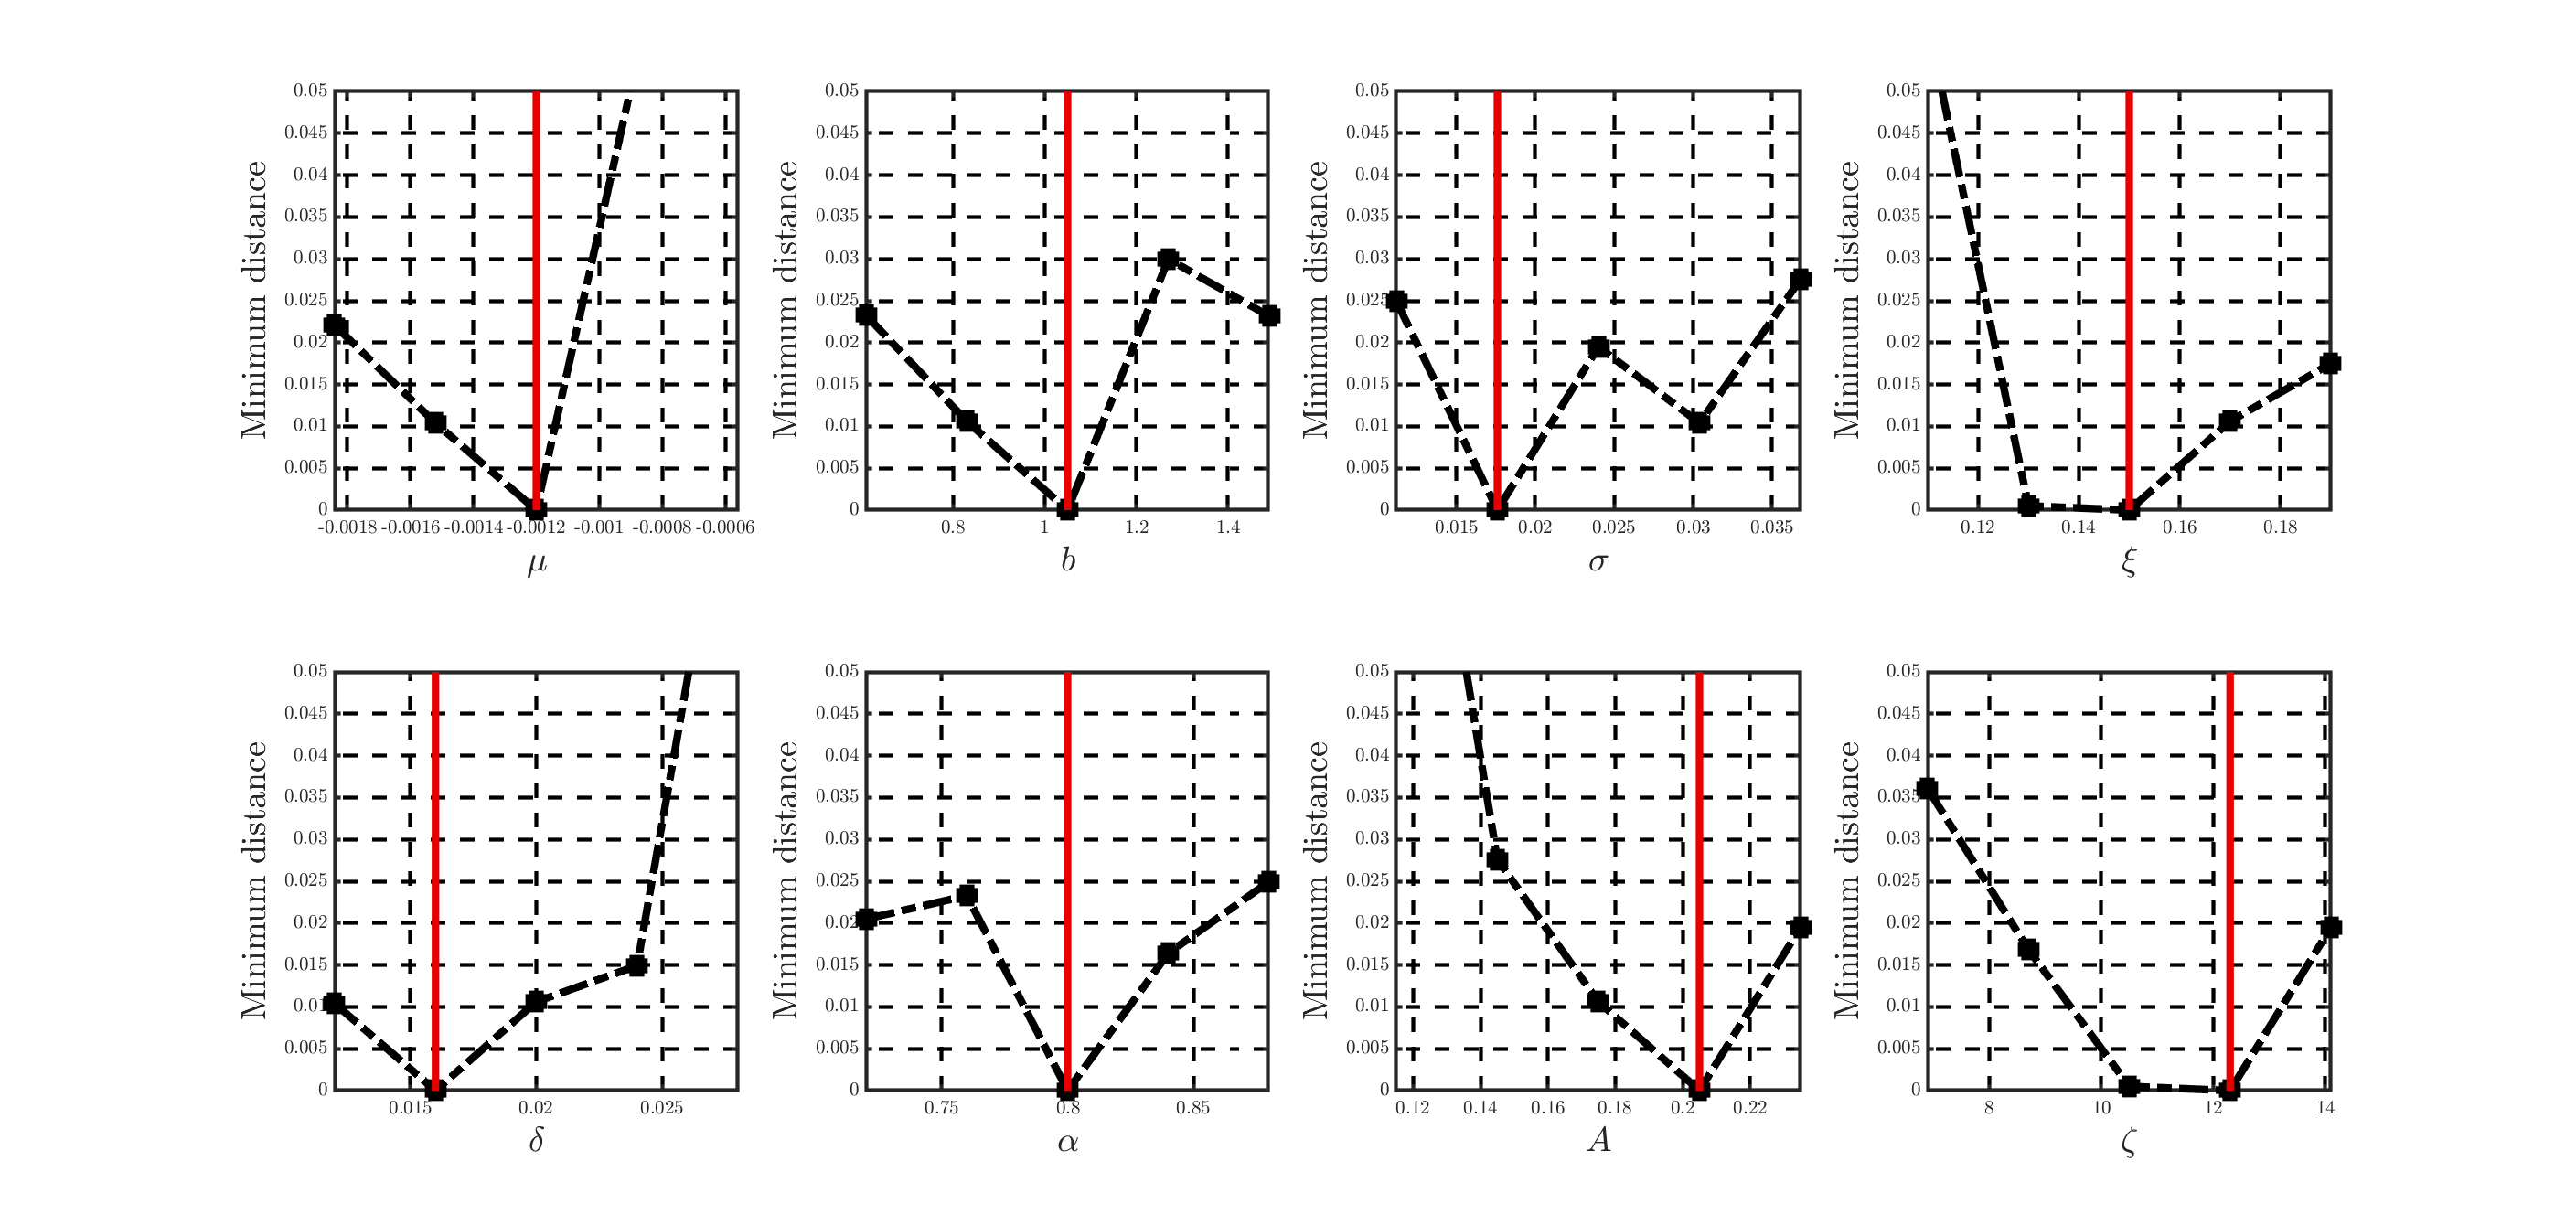
\includegraphics[angle=0,width=16cm]{\MATLABfigureDir/FigE1_MinimumDistance_png}
%\vspace*{-1.3cm}
\caption{Minimum distance as function of each parameter}\label{figure: identification_global}\vspace*{-0.3cm}
\end{center}
{
\footnotesize \underline{Notes}
For each parameter $\psi_i\in\{\mu,\dots,b\}$, the black line plots the minimum distance function $\psi_i \mapsto \mathcal{G}(\psi_i,\bm{\psi}_{-i}^*)$, where $\pmb{\psi}_{-i}^*$ adjusts to minimize the distance criterion.
The red vertical line marks the estimated value $\psi_i^\ast$ listed in Table \ref{table: estimated parameters}
}\vspace*{.75cm}
\end{figure}

\begin{figure}[h!]
\begin{center}
\hspace*{-.85cm}
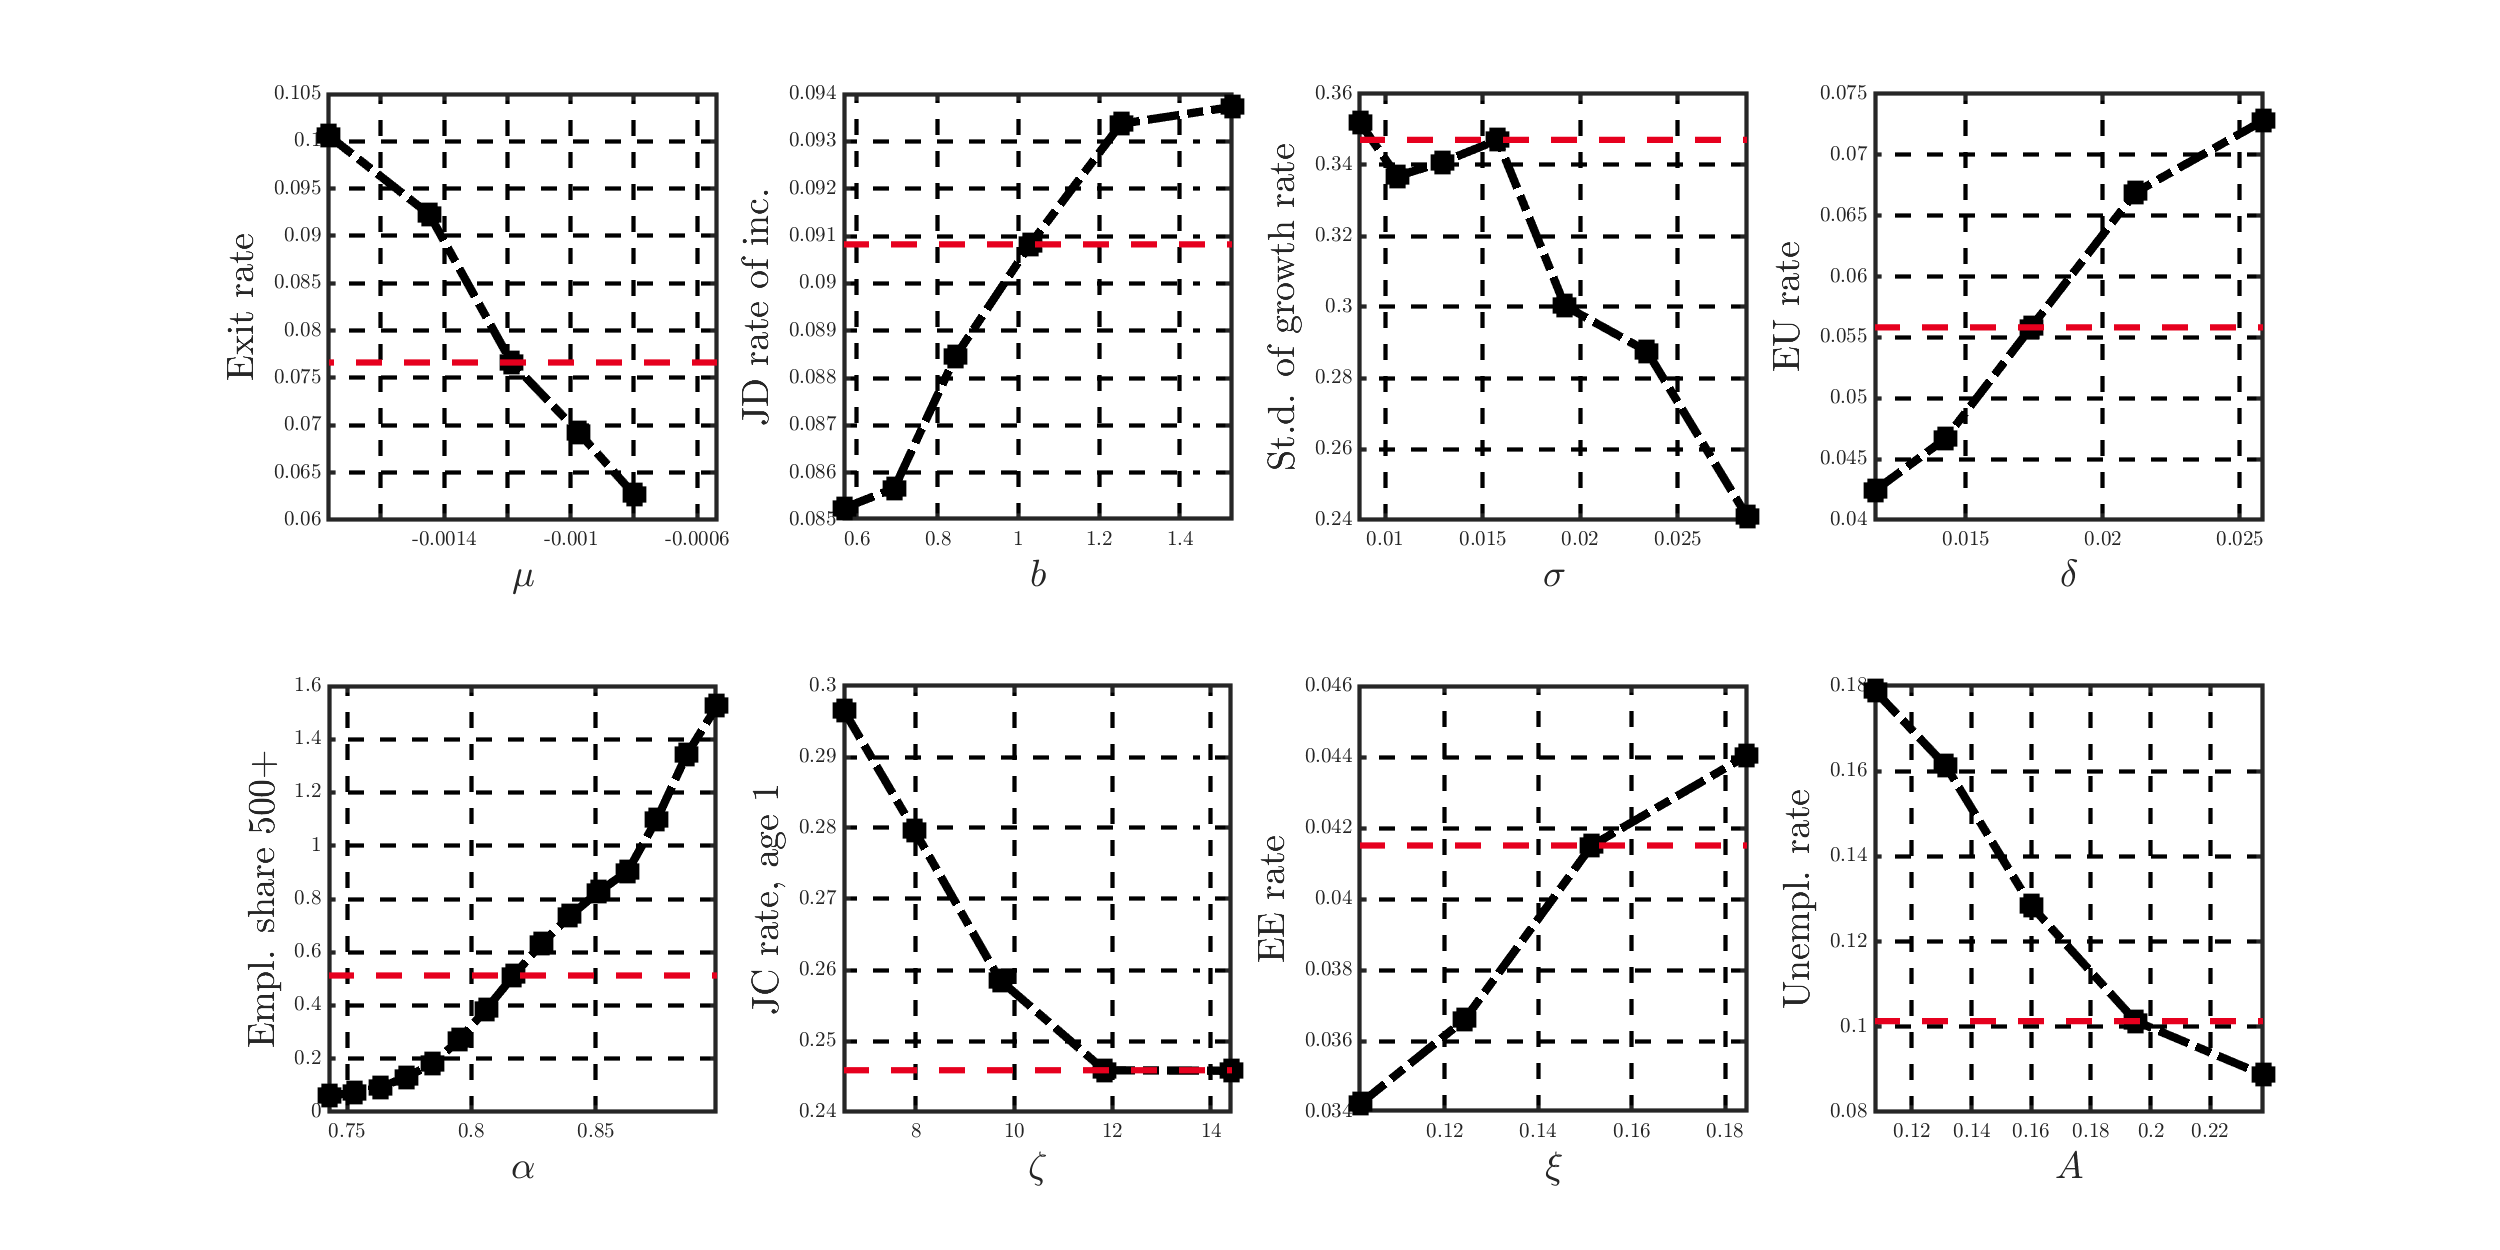
\includegraphics[angle=0,width=16cm]{\MATLABfigureDir/FigE2_TargetMomentsParameters_png}
\caption{Each targeted moment against each parameter}\label{figure: identification_local}\vspace*{-0.3cm}
\end{center}
{\footnotesize \underline{Notes}
This figure plots the relationship between each parameter $\psi_i\in \{\mu,\dots,b\}$ and the moment aligned with the
parameter in Table \ref{table: estimated parameters}.
For each panel, the $x$-axis plots alternative values of the parameter.
The $y$-axis plots the change in the corresponding moment in the steady state of the model obtained when all other parameters are as in Table  \ref{table: estimated parameters}.
}
\end{figure}



